\section{Captive Portal - Proof of Concept}
\label{section:realisation:captive_portal}
\subsection{Lastenheft}
Nach dem Treffen mit PulseShift am 08.03 wurde ein Lastenheft mit den folgenden Punkten ausgearbeitet:
\begin{itemize}
\item Es soll ein Captive Portal innerhalb eines WLAN Netzwerks eingerichtet werden, das die Nutzer optional zu einer Umfrage weiterleiten kann.
\item Es sollen mehrere Hardwarelösungen mit Captive Portal Funktionalität, wie ein Raspberry Pi, ein Router oder ein Accesspoint, untersucht werden. 
\item Dabei sollen Hersteller-agnostische Lösungen gefunden werden.
\item Anschließend soll das Captive Portal durch genau eine der untersuchten Hardwarelösungen realisiert werden.
\item Die dabei benötigte Hardware soll unter Absprache mit Pulseshift von Pulseshift organisiert werden.
\item Der Nutzer, der ein Endgerät mit dem erzeugten WLAN Netzwerk verbindet, soll über die Möglichkeit zur Teilnahme an einer Umfrage informiert, jedoch nicht gezwungen werden.
\item Durch einen Redirect soll der Nutzer direkt zu einer Umfrageseite gelangen, die die Fragebögen von Pulseshift beinhaltet.
\item Die Fragebögen von Pulseshift sollen entweder lokal auf der Hardwarelösung gespeichert sein oder über das Internet direkt angesteuert werden.
\end{itemize}

\subsection{Pflichtenheft}
Anhand des zuvor erarbeiteten Lastenhefts wurde anschließend ein Pflichtenheft mit folgendem Inhalt erstellt:
\begin{itemize}
\item Es werden Hardwarelösungen mit Captive Portal Funktionalität untersucht.
\item Dabei werden Router, Accesspoints und Rasbperry Pis genauer behandelt.
\item Die Anwendungsmöglichkeiten, Vor- \& Nachteile der einzelnen Komponenten wird erarbeitet.
\item Als weiteres Auswahlkriterium wird überprüft ob eine entsprechende Lösung unabhängig vom Hersteller der Hardware erfolgen kann.
\item Unter Absprache mit Pulseshift wird eine entsprechende Hardwarelösung von Pulseshift bereitgestellt.
\item Die gegebene Hardwarelösung wird ein WLAN Netzwerk erzeugen, indem sich Nutzer, die sich in unmittelbarer Nähe befinden, mit ihren Endgeräten anmelden können.
\item Ein Nutzer, der in diesem Netzwerk angemeldet ist, wird über die freiwillige Teilnahmemöglichkeit an einer Umfrage von Pulseshift informiert.
\item Diese Information wird in Form eines Popups auf dem entsprechenden Endgerät erscheinen.
\item Das Popup wird zwei Optionen beinhalten, die Option zur Umfrage zu gelangen und die Option nicht an der Umfrage teilzunehmen.
\item Erstere Option wird entweder per Internet direkt zu der von Pulseshift gehosteten Umfrage führen oder eine auf der Hardwarelösung lokal gespeicherte Kopie der Fragebögen anzeigen.
\item Insofern die Umfrage lokal gespeichert ist und kein Internetzugang vorhanden ist, werden die angegebenen Antworten und Informationen des Nutzers ebenfalls lokal gespeichert.
\item Die zweite Option wird das Popup schließen.
\end{itemize}

\subsection{EPK: Ablauf der Anwendung}
\begin{figure}[H]
\centering
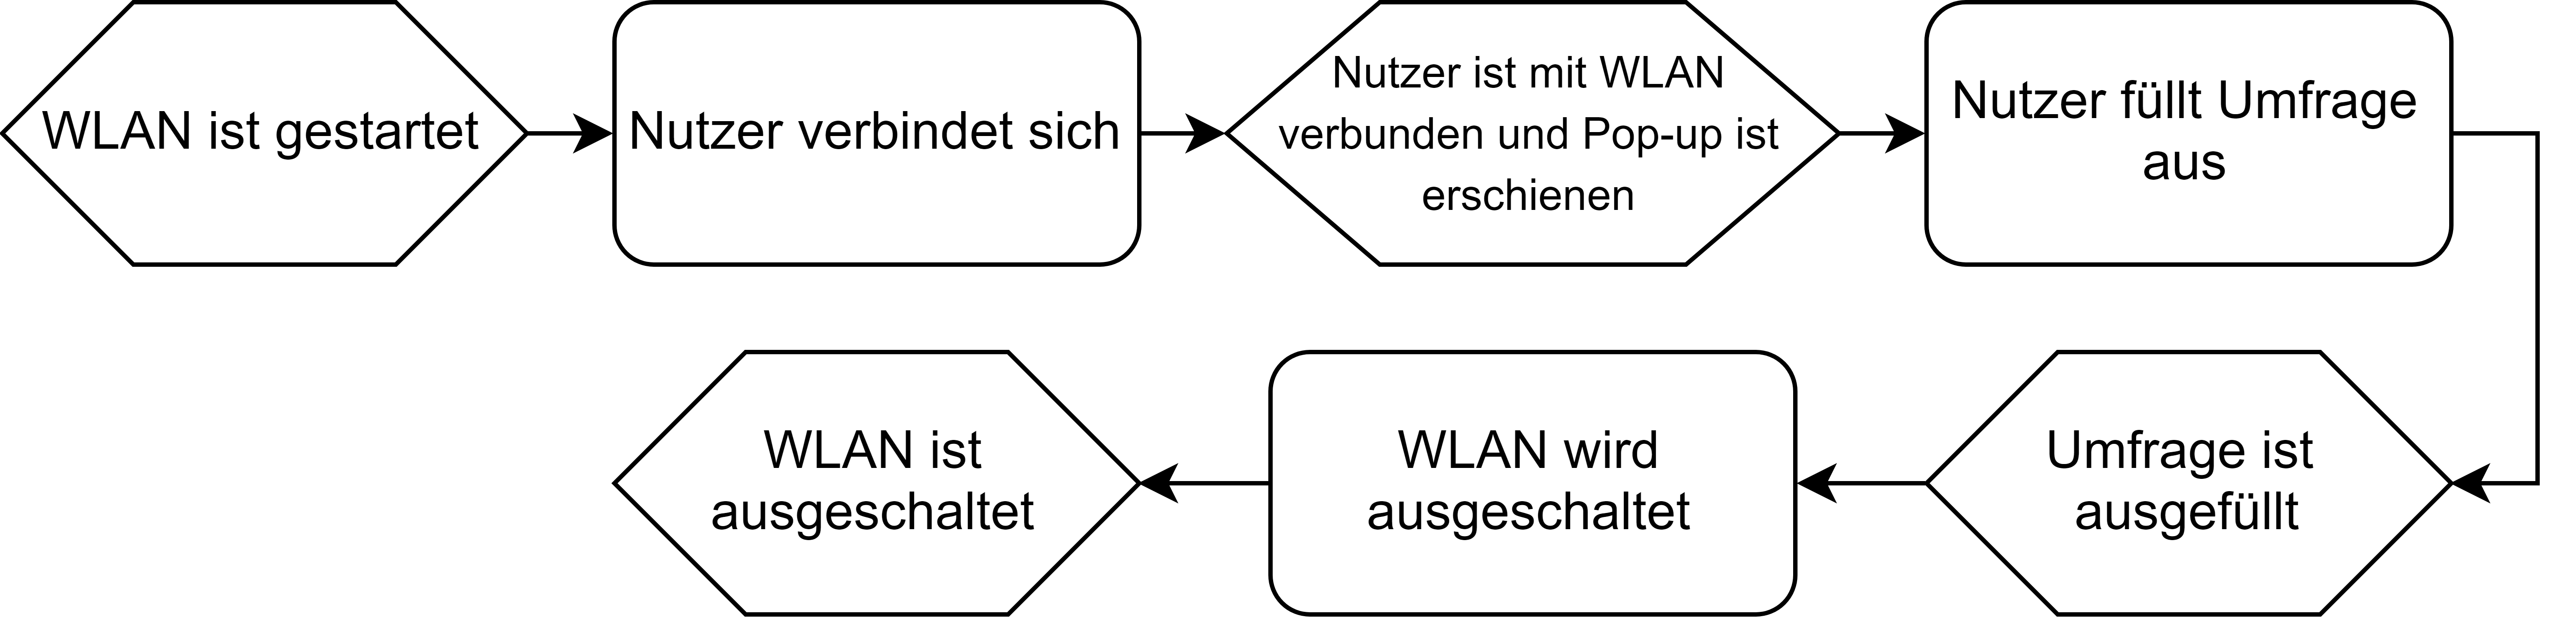
\includegraphics[width=0.9\textwidth]{images/captiveportal_EPK1}
\caption[EPK zum Ablauf ohne Internetzugang]{EPK zum Ablauf ohne Internetzugang}
\end{figure}

\begin{figure}[H]
\centering
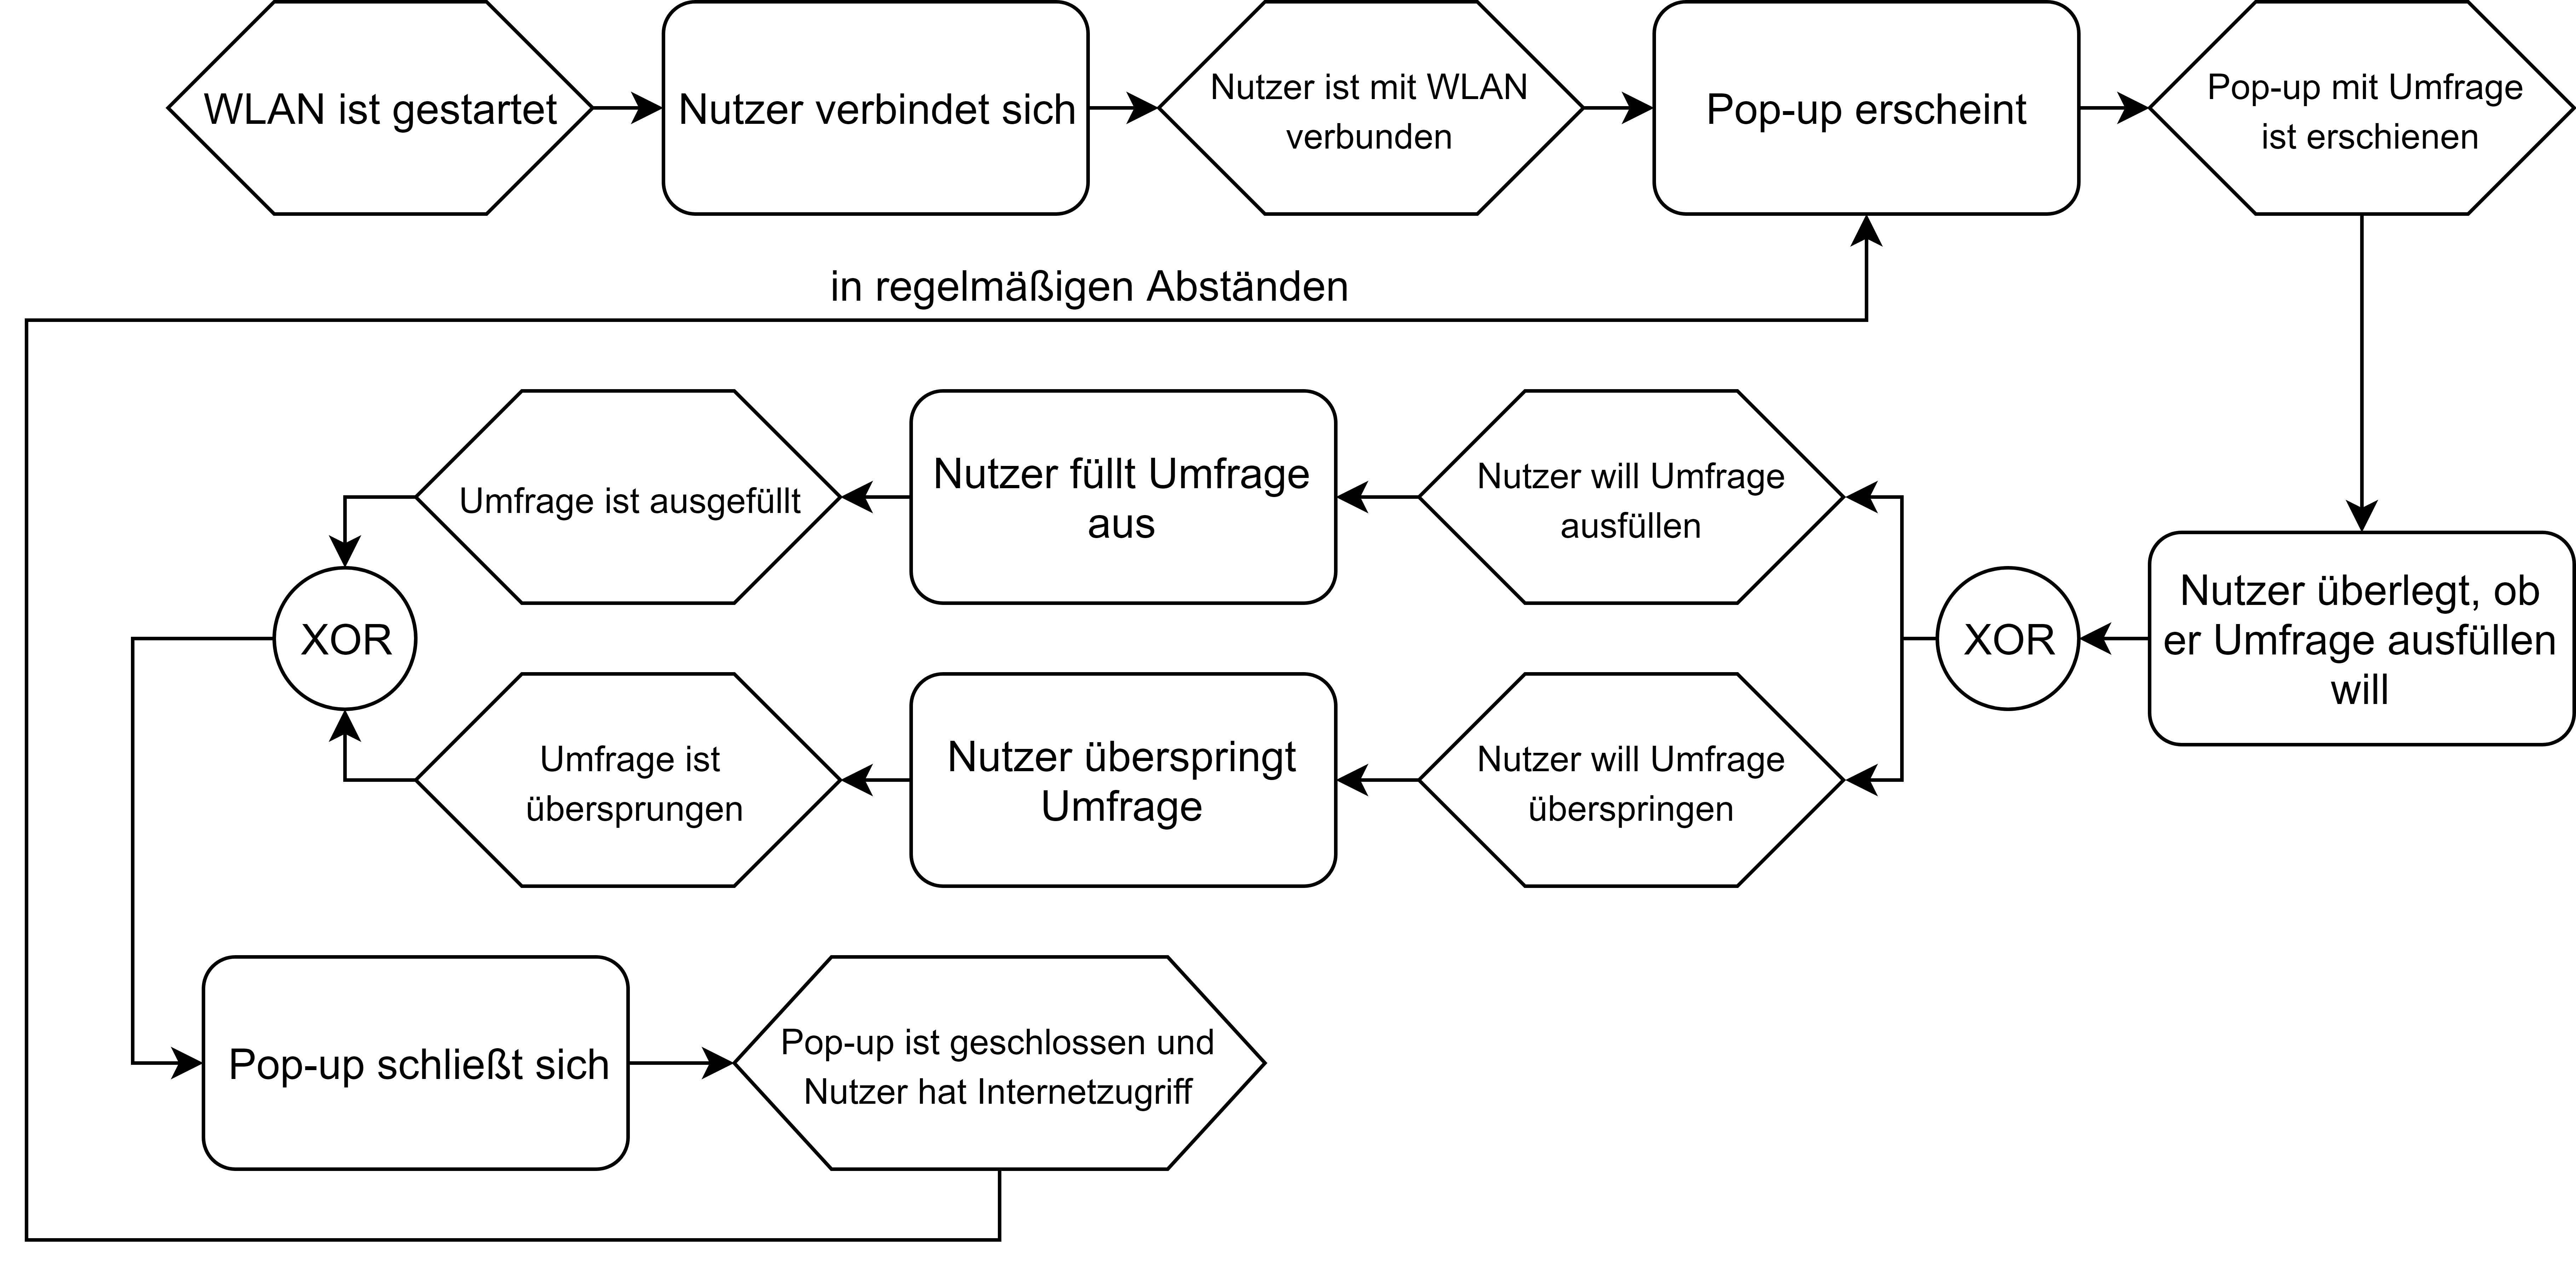
\includegraphics[width=0.9\textwidth]{images/captiveportal_EPK2}
\caption[EPK zum Ablauf mit Internetzugang]{EPK zum Ablauf mit Internetzugang}
\end{figure}
\subsection{Architektur}
\subsubsection{Verwendung eines Raspberry Pi}
\subsubsection*{Initiale Einrichtung und verwendete Hardware}
Der Raspberry Pi soll die Funktionalität eines Captive Portals für Umfragen veranschaulichen. Grundsätzlich benötigt wird hierfür:
\begin{itemize}
\item Raspberry Pi 3
\item Stromkabel
\item SD Karte
\end{itemize}

Da der Raspberry Pi 3 bereits einen WLAN-Empfänger eingebaut hat, wird kein zusätzlicher - etwa über USB - benötigt. Zunächst muss das Betriebssystem Raspbian Stretch auf dem Raspberry Pi  installiert werden. Hierfür kann beispielsweise das Installationsprogramm \textit{NOOBS} genutzt werden, das über einen Computer auf die SD Karte gespielt wird. Anschließend erfolgt die Installation und die Aktualisierung des Betriebssystems durch \textit{apt-get update} und \textit{apt-get upgrade}.

\subsubsection*{Anleitung 1 - Captive Portal ohne Internet}
Um das Captive Portal einzurichten, wird zunächst der Ansatz ohne Internetverbindung, also mit einer lokal gehosteten Webseite, gewählt. Hierfür wird der unter \textit{https://brennanhm.ca/knowledgebase/2016/10/raspberry-pi-access-point-and-captive-portal-without-internet/} zu findenden Anleitung gefolgt. Hierbei müssen auf dem Raspberry Pi die Pakete \textit{hostapd} und \textit{dnsmasq} installiert werden.

Das Paket \textit{hostapd} ermöglicht es, dass der WLAN-Empfänger als Access Point dienen kann, also Verbindungen von anderen Endgeräten annimmt. Bei dem Paket \textit{dnsmasq} handelt es sich um einen einfach zu konfigurierenden DNS- und DHCP-Server. Für beide Pakete müssen anschließend weitere Konfigurationen durchgeführt werden.

Das letzte Paket \textit{nginx} bietet einen Webserver, der für das lokale Hosting der Umfrage-Sseite genutzt wird. Die in der Anleitung vorgeschlagene \textit{nginx} Konfiguration wird um das rewrite-Statement für den /feedback/ Pfad ergänzt. In dem Block für den /generate\_204 Pfad können URL-Parameter mitzurückgegeben werden. Diese werden auch auf Android und auf Windows Endgeräten genutzt, bei iOS hingegen funktioniert dies nicht. Aus diesem Grund wurden diese URL-Parameter, nach unterschiedlichen Versuchen, nginx richtig zu konfigurieren, direkt in der JavaScript-Datei der Umfrage-Webseite einmalig festgelegt.

Das Captive Portal des Raspberry Pi funktioniert mit dieser Anleitung problemlos auf Windows-Computern, iOS-Endgeräten und den meisten Android-Engeräten. Lediglich bei Samsung-Smartphones öffnet sich der Pop-up zum Anmelden am WLAN nicht. Der Grund hierfür ist nicht klar, könnte jedoch möglicherweise durch eine andere dnsmasq- oder nginx-Konfiguration behoben werden.

Die automatische Einrichtung des Raspberry Pi wird durch ein selbst erstellten Shell Skript ermöglicht, dass die Schritte in der Anleitung hintereinander durchführt. Voraussetzung ist ein neu aufgesetzter Raspberry Pi 3 mit WLAN-Interface wlan0. Der Name des WLANs wird als Argument \textit{sudo bash setup.sh Name\_des\_WLANs} übergeben, die Webseite muss anschließend in den Ordner /usr/share/nginx/html/host kopiert werden.

\subsubsection*{Anleitung 2 - Captive Portal mit Internet}
Eine zweite Anleitung ermöglicht es, den Raspberry Pi als WLAN-Access Point mit Captive Portal für einen Internetzugang zu nutzen, was auch die Verwendung für einen permanenten Einsatz - etwa in einer Kantine - ermöglichen würde. Hierfür werden die Anleitungen 2a unter \textit{https://pimylifeup.com/raspberry-pi-wireless-access-point/} für die Einrichtung des Access Points und 2b unter \textit{https://pimylifeup.com/raspberry-pi-captive-portal/} für die Captive Portal Funktionalität genutzt.

Für die Einrichtung des Access Points werden erneut die Pakete \textit{hostapd} und \textit{dnsmasq} genutzt. Zusätzlich werden noch die IP-Tabellen verändert und diese Veränderungen und ein Neustart von \textit{hostapd} und \textit{dnsmasq} in die rc.local Datei geschrieben, damit diese bei jedem Neustart neu umgesetzt werden. Dies hat jedoch bei dem Austesten der Anleitung nicht funktioniert, sodass ein \textit{sleep 10} Befehl der rc.local Datei hinzugefügt werden musste.

Im zweiten Schritt wird für den Access Point die Captive Portal Funktionalität hinzugefügt. Hierfür wird die Software \textit{nodogsplash} auf dem Raspberry Pi installiert. Diese hostet lokal die Captive Portal Seite in dem Verzeichnis \textit{/etc/nodogsplash/htdocs/splash.html}. Auf der Captive Portal Seite kann ein Formular abgeschickt werden, mit dem der Nutzer authentifiziert wird und mit dem er Zugriff auf das Internet erhält. In der nodogsplash.conf Datei können weitere Konfigurationen vorgenommen werden, insbesondere auch der Internetzugriff für nicht-authentifizierte Nutzer erlaubt werden, sodass auf der Captive Portal Seite Inhalte aus dem Internet angezeigt werden.

Diese Lösung funktioniert auf allen Endgeräten, insbesondere auch auf denen von Samsung. Liegt kein Internet vor, funktioniert das Captive Portal jedoch nicht. Hierfür muss in der dnsmasq.conf Konfigurationsdatei \textit{address=/\#/IP\_des\_Raspberry} hinzugefügt werden, damit alle Domainnamen auf den Raspberry aufgelöst werden. Ist dies erfolgt, funktioniert das automatische Pop-up bei Samsung Smartphones jedoch nicht mehr.

Auch für diese Anleitungen wurde Shell Skript umgesetzt. Diese können mit \textit{sudo bash setup2a.sh Name\_des\_WLANs Passwort\_des\_WLANs} und \textit{sudo bash setup2b.sh} ausgeführt werden.

\subsubsection*{Weiteres Vorgehen}
Die Umsetzung des Captive Portals mithilfe des Raspberry Pi dient in erster Linie zur Veranschaulichung der Möglichkeit, die Umfrage in dieser Form umzusetzen. Sollte eine der Lösungen des Raspberry Pi tatsächlich in einem produktiven Umfeld genutzt werden, sind folgende Aspekte zu beachten:
\begin{itemize}
\item Es müsste ein externer WLAN-Empfänger genutzt werden, da der in dem Raspberry Pi eingebaute Empfänger vermutlich eine zu geringe Signalstärke hat. In diesem Fall müssten die Konfigurationen entsprechend angepasst werden. Gleichzeitig müsste überprüft werden, wie viel Verbindungen gleichzeitig unterstützt werden können.
\item Das Problem der automatischen Pop-ups bei Samsung Handys müsste behoben werden, das Problem liegt womöglich an der DNS-Auflösung oder der zurückgegebenen Status-Codes.
\item Die Anleitungen müssten vertieft auf die Aspekte Sicherheit und Performance überprüft werden, möglicherweise auch eine SSL-Verschlüsselung eingerichtet werden.

\end{itemize}

\subsubsection{Alternative Ansätze}

